\section{Accelerating ROMs of Non-linear Systems}\label{sec:hyperreduction}

So far, we have pointedly ignored the fact that the Galerkin (Eq.~\ref{eq:galerkinROMODE}), LSPG (Eq.~\ref{eq:lspgLSLin}), and MP-LSVT (Eq.~\ref{eq:mplsvtLSLin}) ROMs \textit{will not generate computational cost savings} for large-scale non-linear systems. This is largely due to the fact that evaluating the non-linear terms $\rhsFunc{\cdot}$ arising from fluxes, source terms, body forces, and boundary conditions still scales with the full-order dimension $\numDOF$. Linear time-invariant systems do not suffer from this issue; given a system of the form $\consVecDt - \dummyMat \consVec = \zeroVec$, $\dummyMat \inRTwo{\numDOF}{\numDOF}$, the resulting Galerkin ROM (assuming $\consScale = \resScale = \identMat$) takes the form
%
\begin{equation}
    \ode{\consVecCoef}{\timeVar} = \consTrial^\top \dummyMat \consTrial \consVecCoef.
\end{equation}
%
The matrix $\consTrial^\top \dummyMat \consTrial \consVecCoef \inRTwo{\numConsModes}{\numConsModes}$ can be precomputed in the \textit{offline} stage before evaluating the ROM in the \textit{online} stage. Such a precomputation is impossible for general non-linear systems. The low-dimensional state must first be \textit{lifted} to the full-dimensional state (via $\decoderFunc{\consVecCoef}$) to evaluate the non-linear terms $\rhsFunc{\cdot}$. In the case of Galerkin projection, this term must then be projected onto the tangent trial space before integrating the low-dimensional ODE in time. In the case of LSPG and MP-LSVT ROMs solved via the normal equations, the time-variant test basis must be computed from the residual Jacobian. Despite the fact that the resulting low-dimensional system may be less expensive to temporally integrate, these additional operations often outweigh any cost savings. Particularly for complex multi-physics systems, the evaluation of $\rhsFunc{\cdot}$ accounts for the vast majority of the solver cost, and failing to reduce this cost often fails to reduce the ROM cost below that of the FOM.

To achieve the intended goal of significantly reducing the cost of evaluating the model, we must eliminate the ROM's dependence on the full-order dimension $\numDOF$. Techniques which seek this goal are generally referred to as \textit{hyper-reduction} methods. Most prevalent and mature are so-called \textit{sparse sampling} methods, which evaluate the non-linear terms at a small number of carefully selected degrees of freedom and reconstruct them approximately using data-driven modeling techniques. Work in this thesis focuses on linear sparse-sampling methods for linear subspace ROMs, namely the discrete empirical interpolation method and gappy proper orthogonal decomposition. Neural network approaches to hyper-reduction~\cite{nnHyperRed} and hyper-reduction for non-linear manifold ROMs~\cite{Kim2022} have been proposed, but are not discussed or analyzed here.

\subsection{DEIM and Gappy POD ROMs}
%
Two well-established hyper-reduction methods for projection-based ROMs of discrete dynamical systems are the discrete empirical interpolation method (DEIM) and gappy proper orthogonal decomposition (gappy POD). The two are closely related, but were originally developed for different applications. DEIM, introduced by Chaturantabut and Sorensen~\cite{Chaturantabut2010}, is a discrete formulation of the empirical interpolation method (EIM)~\cite{Barrault2004}. It introduces an approximation of non-linear functions of the form,
%
\begin{equation}\label{eq:deimRHSApprox}
    \resFunc{\consVec} \approx \resApproxFunc{\consVec} \defEq \deimBasis \left[ \sampMat \deimBasis \right]^{-1} \sampMat \resFunc{\consVec},
\end{equation}
%
where $\sampMat = [\canonVec_{\dummyIdx_1}, \; \canonVec_{\dummyIdx_2}, \; \hdots, \; \canonVec_{\dummyIdx_{\numSamps}} ]^\top \inRTwo{\numSamps}{\numDOF}$ is composed of \numSamps\ unique canonical unit vectors $\canonVec_{\dummyIdx} \inROne{\numDOF}$. The operation $\sampMat \resVec \inROne{\numSamps}$ thus selects each $\dummyIdx$th degree of freedom from $\resVec$. The matrix $\deimBasis = [\deimBasisVec_1, \; \deimBasisVec_2, \; \hdots, \; \deimBasisVec_{\numResModes}] \inRTwo{\numDOF}{\numResModes}$ is an orthonormal basis, usually generated by POD from FOM snapshots of the non-linear function $\resVec$. It is assumed that the matrix $\sampMat \deimBasis \inRTwo{\numSamps}{\numResModes}$ has full rank. In computing $\resApproxVec$, we see that the non-linear function $\resVec$ must only be computed, or \textit{sampled}, at $\numSamps$ degrees of freedom, instead of its full dimension $\numDOF$. When $\numSamps \ll \numDOF$, the cost of computing $\resApproxVec$ may be much less than the cost of computing $\resVec$.

Note that here, the number of DEIM basis modes is equal to the number of sampled degrees of freedom, i.e., $\numSamps = \numResModes$. By this formulation, the non-linear function is interpolated exactly at $\numSamps < \numDOF$ degrees of freedom and interpolated approximately at all other degrees of freedom. The error in this approximation is bounded~\cite{Chaturantabut2010} by the inequality
%
\begin{equation}\label{eq:deimErrorBound}
   \left\Vert \resFunc{\consVec} - \resApproxFunc{\consVec} \right\Vert_2 \le \left\Vert \left[ \sampMat \deimBasis \right]^{-1} \right\Vert_2 \left\Vert \left[ \identMat - \deimBasis \deimBasis^\top \right] \resFunc{\consVec} \right\Vert_2,
\end{equation}
%
where the first norm term on the right-hand side is a measure of the \textit{sampling error}, and the second norm term is the \textit{projection error}. As will be discussed shortly, various methods of selecting the sampling degrees of freedom often attempt to minimize these sources of error.

DEIM has been successfully applied to a variety of interesting dynamical systems~\cite{Chaturantabut2011, Henneron2014}, but is quite limited by the restriction $\numSamps = \numResModes$. Recall that for practical engineering systems, $\numResModes \ll \numDOF$ generally, and such extreme sparse sampling may result in high interpolation error at the unsampled degrees of freedom. Furthermore, Peherstorfer et al.~\cite{Peherstorfer2020} show that increasing $\numResModes$ can lead to an unstable increase in the interpolation error.

Gappy POD, originally developed well before the advent of DEIM to approximate full field data from a few sparse samples~\cite{Everson1995}, can also be used to approximate non-linear functions in dynamical systems. The method takes a very similar approach to DEIM, but relaxes the restriction on the number of sampled degrees of freedom, allowing $\numSamps \ge \numResModes$. Thus, the approximation becomes a least-squares regression of the form,
%
\begin{equation}\label{eq:gappyPODRHSApprox}
    \resFunc{\consVec} \approx \resApproxFunc{\consVec} \defEq \deimBasis \left[ \sampMat \deimBasis \right]^{+} \sampMat \resFunc{\consVec},
\end{equation}
%
where the operation $\dummyMat^+$ indicates the Moore--Penrose inverse (or pseudo-inverse). Again, this assumes $\sampMat \deimBasis$ has full rank. Similarly to Eq.~\ref{eq:deimErrorBound}, the gappy POD regression error is bounded by
%
\begin{equation}\label{eq:gappyPODErrorBound}
    \left\Vert \resFunc{\consVec} - \resApproxFunc{\consVec} \right\Vert_2 \le \left\Vert \left[ \sampMat \deimBasis \right]^{+} \right\Vert_2 \left\Vert \left[ \identMat - \deimBasis \deimBasis^\top \right] \resFunc{\consVec} \right\Vert_2.
\end{equation}
%
For the remainder of this thesis, we will restrict discussion of hyper-reduction to gappy POD, as it is more general than DEIM. We simply remind the reader that in the specific case of $\numResModes = \numConsModes$, gappy POD is equivalent to DEIM.

\paragraph*{Hyper-reduction of Galerkin ROMs}\mbox{}\\
%
The approximation of non-linear functions by Eq.~\ref{eq:gappyPODRHSApprox} can be directly applied to projection-based ROM formulations. In the case of Galerkin projection, the non-linear terms $\rhsVec$ may be approximated as
%
\begin{equation}
	\rhsApproxFunc{\consVec, \; \timeVar} \defEq \deimBasis \left[ \sampMat \deimBasis \right]^+ \sampMat \rhsFunc{\consVec, \; \timeVar}.
\end{equation}
%
Substituting this approximation into the Galerkin ROM ODE (Eq.~\ref{eq:galerkinROMODE}) results in the hyper-reduced ROM
%
\begin{equation}\label{eq:galerkinROMHR}
    \ode{\consVecCoef}{\timeVar} = \left[\jacobDecode^\top \resScaleInv \jacobDecode\right]^{-1} \jacobDecode^\top \resScaleInv \deimBasis \left[ \sampMat \deimBasis \right]^+ \sampMat \rhsFunc{\consVecRom, \; \timeVar}.
\end{equation}
%
With a linear trial space, recall that $\jacobDecode = \consScale \consTrial$. This results in the simplified formulation
%
\begin{equation}
    \ode{\consVecCoef}{\timeVar} = \left[\consTrial^\top \consScale \resScaleInv \consScale \consTrial\right]^{-1} \consTrial^\top \consScale \resScaleInv \deimBasis \left[ \sampMat \deimBasis \right]^+ \sampMat \rhsFunc{\consVecRom, \; \timeVar}.
\end{equation}
%
The low-dimensional matrix $\left[\consTrial^\top \consScale \resScaleInv \consScale \consTrial\right]^{-1} \consTrial^\top \consScale \resScaleInv \deimBasis \left[ \sampMat \deimBasis \right]^+ \inRTwo{\numConsModes}{\numSamps}$ can be pre-computed in the offline stage and loaded from disk prior to evaluating the unsteady ROM. Futher simplifying, if $\consScale = \resScale = \identMat$, the formulation is greatly reduced to
%
\begin{equation}
    \ode{\consVecCoef}{\timeVar} = \consTrial^\top \deimBasis \left[ \sampMat \deimBasis \right]^+ \sampMat \rhsFunc{\consVecRom, \; \timeVar},
\end{equation}
%
where again, the low-dimensional matrix $\consTrial^\top \deimBasis \left[ \sampMat \deimBasis \right]^+ \inRTwo{\numConsModes}{\numSamps}$ can be precomputed. {\color{red}Add some citations of applications}

\paragraph*{Hyper-reduction of LSPG and MP-LSVT ROMs}\mbox{}\\
%
Applying gappy POD to LSPG and MP-LSVT ROMs takes a slightly different approach than that used for Galerkin ROMs. Instead of constructing a least-squares regression for the non-linear function $\rhsVec$, the complete fully-discrete residual $\resVec$ is approximated, as in Eq.~\ref{eq:gappyPODRHSApprox}, and substituted into the residual minimization problem given by Eq.~\ref{eq:lspgLS} or~\ref{eq:mplsvtLS}. We first examine the procedure for LSPG, which was first formulated by Carlberg and coworkers~\cite{Carlberg2010,Carlberg2013}, who referred to the procedure as Gauss--Newton with approximated tensors (GNAT). Substituting the residual approximation into Eq.~\ref{eq:lspgLS} results in the non-linear least-squares problem
%
\begin{equation}\label{eq:lspgLSHR}
    \consVecCoef^{\timeIdx} = \argmin{\dummyVec \inROne{\numConsModes}} \left\Vert \resScaleInv \deimBasis \left[ \sampMat \deimBasis \right]^{+} \sampMat \resFunc{\dummyVec} \right\Vert_2.
\end{equation}
%
Solving Eq.~\ref{eq:lspgLSHR} by Gauss--Newton results in the iterative process
%
\begin{equation}\label{eq:lsgpLinHR}
    \delta \consVecCoef^{\newtonIdx} = \argmin{\dummyVec \inROne{\numConsModes}} \left\Vert \resScaleInv \deimBasis \left[ \sampMat \deimBasis \right]^{+} \left(\sampMat \jacobRes^{\newtonIdx} \dummyVec - \sampMat \resFunc{\consVecCoef^{\newtonIdx}}\right) \right\Vert_2,
\end{equation}
\begin{equation}
    \consVecCoef^{\newtonIdx + 1} = \consVecCoef^{\newtonIdx} + \alpha \left[ \delta \consVecCoef^{\newtonIdx} \right].
\end{equation}
%
Solution of Eq.~\ref{eq:lsgpLinHR} via the normal equations is again given by a Petrov--Galerkin ROM of the form
%
\begin{equation}\label{eq:lspgHRSolve}
    \left[ \testBasisCons^\newtonIdx \right]^\top \testBasisCons^\newtonIdx \delta \consVecCoef^{\newtonIdx} = -\left[\testBasisCons^\newtonIdx \right]^\top \resScaleInv \deimBasis \left[ \sampMat \deimBasis \right]^{+} \sampMat \resFunc{\consVecCoef^{\newtonIdx}}.
\end{equation}
%
where the test basis is defined as
%
\begin{equation}\label{eq:lspgHRTest}
    \testBasisCons^\newtonIdx \defEq \resScaleInv \deimBasis \left[ \sampMat \deimBasis \right]^{+} \sampMat \jacobCons^{\newtonIdx} \jacobDecode^{\newtonIdx}.
\end{equation}
%

Hyper-reduction of MP-LSVT ROMs via gappy POD follow an extremely similar method, beginning from the fully-discrete residual minimization with respect to the target state latent variables,
%
\begin{equation}
    \primVecCoef^{\timeIdx} = \argmin{\dummyVec \inROne{\numPrimModes}} \left\Vert \resScaleInv \deimBasis \left[ \sampMat \deimBasis \right]^{+} \sampMat \resFunc{\dummyVec} \right\Vert_2
\end{equation}
%
Solution via Gauss--Newton and the normal equations results in a similar hyper-reduced Petrov--Galerkin formulation of
%
\begin{equation}\label{eq:mplsvtHRSolve}
    \left[ \testBasisPrim^\newtonIdx \right]^\top \testBasisPrim^\newtonIdx \delta \primVecCoef^{\newtonIdx} = -\left[\testBasisPrim^\newtonIdx \right]^\top \resScaleInv \deimBasis \left[ \sampMat \deimBasis \right]^{+} \sampMat \resFunc{\primVecCoef^{\newtonIdx}},
\end{equation}
%
with the test basis
%
\begin{equation}\label{eq:mplsvtHRTest}
    \testBasisPrim^\newtonIdx \defEq \resScaleInv \deimBasis \left[ \sampMat \deimBasis \right]^{+} \sampMat \jacobPrim^{\newtonIdx} \jacobDecode^{\newtonIdx}.
\end{equation}
%
Only $[ \sampMat \deimBasis ]^{+} \inRTwo{\numResModes}{\numSamps}$ is pre-computed off-line. Although the matrix $\deimBasis [ \sampMat \deimBasis ]^{+} \inRTwo{\numDOF}{\numSamps}$ can be pre-computed off-line, a matrix of $\numDOF \times \numSamps$ elements can be prohibitively large for high-dimensional systems and may not be possible to store in memory.

In Eqs.~\ref{eq:lspgHRSolve} and~\ref{eq:mplsvtHRSolve}, we see that computing the sampled residual $\sampMat \resFunc{\cdot}$ only requires that the residual be evaluated at $\numSamps$ degrees of freedom. Further, in Eqs.~\ref{eq:lspgHRTest} and~\ref{eq:mplsvtHRTest} we see that only the corresponding $\numSamps$ rows of the residual Jacobians $\sampMat $ and $\sampMat$ need to be computed. Thus, the hyper-reduced ROM is truly independent of the FOM dimension $\numDOF$. When $\numSamps \ll \numDOF$ and evaluation of the non-linear terms accounts for a majority of the computational burden, this sparse sampling has the potential to drastically reduce the cost of the hyper-reduced ROM relative to the FOM. Up to four orders of magnitude cost reduction has been recorded, consuming a few core-seconds to compute a ROM where the equivalent FOM simulation might consume many core-hours. Such cost savings bring projection-based ROMs into the realm of possibility for many-query applications.

% Finally, we re-emphasize that traditional approaches to approximating non-linear functions by DEIM and gappy POD have computed \deimBasis\ from FOM time snapshots of the non-linear function being approximated~\cite{sorensen_deim, carlberg_gnat}. This is immediately intuitive, as DEIM and gappy POD seek to approximate the non-linear function. However, we take a slightly different approach in this work, instead using the trial basis computed from the state snapshots to compute the regression as well, i.e., $ \deimBasis = \trialBasisPrim$. Although similar approaches have been successfully employed in past research~\cite{Astrid2008}, this approach is not typically used by DEIM/gappy POD ROM practitioners. Curiously, early investigations by the authors revealed that this decision yields accurate and robust hyper-reduced SP-LSVT ROMs. The reason for this is not yet clearly understood, but will be the subject of future research.

\subsection{Regression Basis Calculation}

\subsection{Sample Selection}

As described above, the computation of the non-linear function regression basis $\deimBasis$ is somewhat nuanced, but is ultimately derived from the POD of a snapshot matrix. Methods for selecting sampling indices, and hence the construction of the sampling operator $\sampMat$, however, are much more varied. The selection of $\numSamps > \numResModes$ samples which globally minimize the regression error (Eq.~\ref{eq:gappyPODErrorBound}) is a computationally-intractable problem. As such, almost all methods for selecting sampling points are \textit{greedy} methods, which iteratively select points based on some measure of local optimality at a given iteration. The ``best'' choice of local error measure, and hence greedy sampling method, is an area of active research. Unfortunately, very few comparisons between sampling methods have been published, with the exception of the work by Peherstorfer \textit{et al.}~\cite{Peherstorfer2020}. Although extremely insightful, their exploration of hyper-reduced ROMs was limited to a simple one-dimensional model problem. Results presented in Chapter~\ref{chap:CavityAndCVRC} seek to expand on their work by studying more complex, 2D and 3D multi-scale and multi-physics problems. In this thesis, we study DEIM greedy sampling (\textit{GappyPOD+D}), random sampling (\textit{GappyPOD+R}), and eigenvector-based sampling (\textit{GappyPOD+E}), which are detailed in turn.

\vspace{0.5cm}
\noindent \textit{GappyPOD+D}:
The GappyPOD+D strategy follows the greedy sampling method originally proposed for DEIM~\cite{Chaturantabut2010} and extended to gappy POD by several researchers~\cite{Zhou2012,Carlberg2013}. This method seeks to minimize the error in computing the regression of the basis vectors $\deimBasisVec_{\dummyIdx}$ themselves. Following a greedy approach, at each sampling iteration $\greedyIdx$ the regression error is calculated by
%
\begin{equation}
    \errVec_{\greedyIdx} = \deimBasisVec_{\dummyIdx} - \deimBasis_{\dummyIdxTwo} \left[ \sampMat_{\greedyIdx} \deimBasis_{\dummyIdxTwo} \right]^+ \sampMat_{\greedyIdx}\deimBasisVec_{\dummyIdx},
\end{equation}
%
where the index $\dummyIdx$ repeatedly loops through the integer interval $\{1, \hdots, \; \numResModes\}$ (the greedy element of this approach), and $\deimBasis_{\dummyIdxTwo} \inRTwo{\numDOF}{\dummyIdxTwo}$ contains the leading $\dummyIdxTwo$ basis vectors of $\deimBasis$. The index $\dummyIdxTwo$ begins at 1 and is incremented by one at every sampling loop, until $\dummyIdxTwo = \numResModes$. At every iteration, the degree of freedom for which the absolute error $|\errVec_{\greedyIdx}|$ is greatest is sampled, and the corresponding canonical unit vector appended to $\sampMat_{\greedyIdx}$. For DEIM interpolations, Chaturantabut and Sorensen~\cite{Chaturantabut2010} showed that this algorithm limits the growth of the error bounds in Eq.~\ref{eq:deimErrorBound} at every iteration $\greedyIdx$.

\vspace{0.5cm}
\noindent \textit{GappyPOD+R}:
For the GappyPOD+R method, the first $\numResModes$ samples are selected by the rank-revealing QR factorization of $\numResModes$. The first $\numResModes$ pivots of the factorization are chosen as sampling points. This \textit{QDEIM} procedure, proposed by Drma\v{c} and Gugercin~\cite{Drmac2016}, has been shown to exhibit tighter error bounds on the resulting interpolant over the traditional DEIM greedy sampling procedure. It has the added benefit of being easily implemented using existing high-performance, parallel linear algebra software libraries.

Selecting the remaining $\numSamps - \numResModes$ samples via the GappyPOD+R strategy is extremely straightforward, as they are simply selected randomly from a discrete uniform distribution. Peherstorfer \textit{et al.}~\cite{Peherstorfer2020} provide probabilistic analyses to show that randomized oversampling limits the growth in regression error as the regression dimension $\numResModes$ is increased, even in the presence of additional system noise.

\vspace{0.5cm}
\noindent \textit{GappyPOD+E}:
The GappyPOD+E method also uses the QDEIM technique as in GappyPOD+R to select the first $\numResModes$ samples. Following this step, the approach seeks to minimize the sampling error term in Eq.~\ref{eq:gappyPODErrorBound} via a greedy approach. This method is a simplification by Peherstorfer et al.~\cite{Peherstorfer2020} of a greedy sampling procedure by Zimmermann and Willcox~\cite{Zimmermann2016} (Algorithm 4), who originally developed the method in the context of missing point estimation. Some of the motivating theory behind the modified algorithm is reproduced here with permission.

To select the remaining $\numSamps - \numResModes$ points, GappyPOD+E leverages the fact that by nature of the $\ell^2$ norm, the sampling error may be rewritten as
%
\begin{equation}
    \left\Vert \left[ \sampMat \deimBasis \right]^+ \right\Vert_2 = \singVal_{\text{max}} \left( \left[\sampMat \deimBasis \right]^+ \right) = \frac{1}{\singVal_{\text{min}} \left( \sampMat \deimBasis \right)},
\end{equation}
%
where $\singVal_{\text{max}}$ and $\singVal_{\text{min}}$ indicate the maximum and minimum singular values of their arguments, respectively. Thus, at each sampling iteration $\greedyIdx$ of the GappyPOD+E method, the row of \deimBasis\ is selected which maximizes the smallest singular value (equivalently, the smallest eigenvalue) of $\sampMat_{\greedyIdx} \deimBasis \inRTwo{\greedyIdx}{\numResModes}$ via a symmetric rank-one update. Here, $\sampMat_{\greedyIdx} \inRTwo{\numDOF}{\greedyIdx}$ is the selection matrix constructed from the $\greedyIdx$ unit vectors selected up to iteration $\greedyIdx$ by the greedy procedure. It is shown in~\cite{Peherstorfer2020} that the bounds on this update of the smallest eigenvalue, $\eigenVal_{\numResModes}$, from update step $\greedyIdx$ to $\greedyIdx+1$, is given by
%
\begin{equation}\label{eq:gappyPODEStrictBounds}
    \eigenVal_{\numResModes}^{\greedyIdx+1} \ge \eigenVal_{\numResModes}^{\greedyIdx} + \frac{1}{2} \left( g + \left\Vert \deimBasisREvecRow \right\Vert_2^2 - \sqrt{\left( g + \left\Vert \deimBasisREvecRow \right\Vert_2^2 \right)^2 - 4g\left( \left[\mathbf{z}_{\numResModes}^{\greedyIdx} \right]^\top \deimBasisREvecRow \right)^2} \right),
\end{equation}
%
where $g = \eigenVal_{\numResModes-1}^{\greedyIdx} - \eigenVal_{\numResModes}^{\greedyIdx}$, and $\mathbf{z}_{\numResModes}^{\greedyIdx} \inROne{\numResModes}$ is the eigenvector associated with eigenvalue $\eigenVal_{\numResModes}^{\greedyIdx}$ (simply the $\numResModes$th canonical unit vector here). Here, $\deimBasisREvecRow = \rightEvecMat_{\greedyIdx}^\top \deimBasisRowUpdate^\top \inROne{\numResModes}$ is defined for simplification, where $\rightEvecMat_{\greedyIdx}$ are the right singular vectors of $\sampMat_{\greedyIdx}^\top \deimBasis$, and $\deimBasisRowUpdate \inRTwo{1}{\numResModes}$ is the row of $\deimBasis$ to be included at greedy iteration $\greedyIdx$. Previous pre-print versions of~\cite{Peherstorfer2020} offer a simplification of the bound in Eq.~\ref{eq:gappyPODEStrictBounds}, given by
%
\begin{equation}\label{eq:gappyPODESimpleBounds}
    \eigenVal_{\numResModes}^{\greedyIdx+1} \ge \eigenVal_{\numResModes}^{\greedyIdx} + \frac{g \left( [\mathbf{z}_{\numResModes}^\greedyIdx]^\top \deimBasisREvecRow \right)^2}{g + \left\Vert \deimBasisREvecRow \right\Vert_2^2}.
\end{equation}
%
Maximizing this bound on $\eigenVal_{\numResModes}^{\greedyIdx+1}$ is thus equivalent to choosing the basis row $\deimBasisRowUpdate$ which maximizes $(\mathbf{z}_{\numResModes}^{\greedyIdx})^\top \deimBasisREvecRow$ at each greedy iteration. In this work, we choose to follow the bounds in Eq.~\ref{eq:gappyPODESimpleBounds}, in contrast to the bounds in Eq.~\ref{eq:gappyPODEStrictBounds}, as the former leads to a simpler algorithm which is more efficient when working with high-dimensional data in a distributed-memory setting. The algorithm for this approach can be found in previous pre-print versions of~\cite{Peherstorfer2020}.

\subsection{The Sample Mesh}

For multi-variate, coupled systems of equations (such as those describing fluid flow systems), sampling individual degrees of freedom of a non-linear function is not equivalent to sampling the state variable arguments associated with those degrees of freedom, e.g., $\sampMat \resFunc{\consVec} \neq \resFunc{\sampMat \consVec}$. Specifically, the evaluation of the non-linear function at a specific degree of freedom often requires access to all state variables at that point in space. For example, solving the continuity equation of the Navier-Stokes equations at a single discrete point in space requires access to both the density and the velocity field. Further, the state at entirely different points in space may also need to be sampled, e.g., to correctly compute fluxes or gradients.

We visualize this in Fig.~\ref{fig:IBlankConfig} in the context of a cell-centered finite volume discretization with quadrilateral/hexahedral control volumes, with a second-order accurate flux scheme. In this image, the blue cell indicates a control volume where at least one degree of freedom of the non-linear function is to be computed. We refer to this type of cell as a \textit{directly sampled} cell. Red cells, or \textit{flux} cells, are those which share a cell face with directly sampled cells and are required for computing fluxes through the shared faces. Yellow cells are those which are required for computing gradients for second-order state reconstructions at cell faces, or for reconstruction of the state at directly sampled cell vertices. These are referred to as \textit{gradient/vertex} cells. We refer to the flux and gradient/vertex cells as \textit{auxiliary} cells, as they are required for calculating the directly sampled degrees of freedom but are not directly sampled themselves. For two-dimensional simulations, each directly sampled cell is accompanied by four flux cells and eight gradient/vertex cells. For three-dimensional simulations, this increases to six flux cells and 26 gradient/vertex cells per directly sampled cell.

\begin{figure}
    \centering
    \begin{minipage}{0.45\linewidth}
        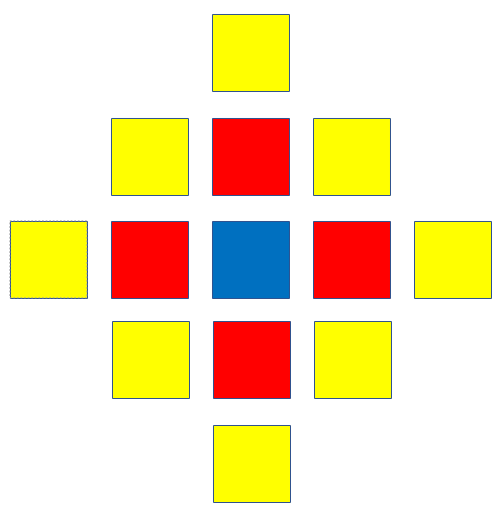
\includegraphics[width=0.99\linewidth]{Chapters/ProjROMs/Images/sampling_2d_2ndOrder.png}
    \end{minipage} \hspace{0.5em}
    \centering
    \begin{minipage}{0.52\linewidth}
        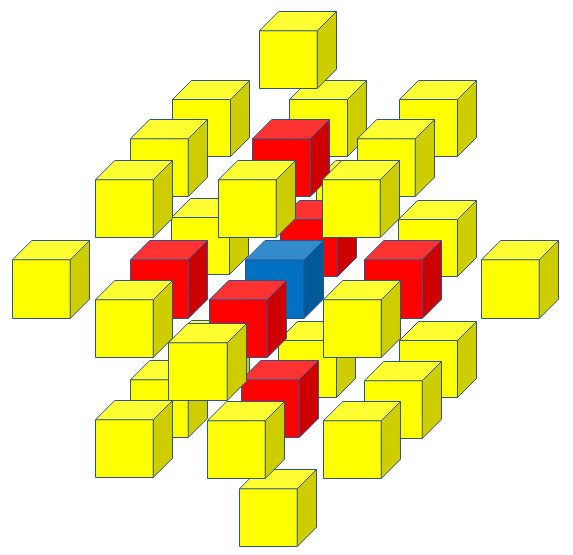
\includegraphics[width=0.99\linewidth]{Chapters/ProjROMs/Images/sampling_3d_2ndOrder.png}
    \end{minipage}
    \caption{\label{fig:IBlankConfig}Sampling schemes for 2nd-order flux scheme in 2D (left) and 3D (right).\\Blue cells are directly sampled, red are flux cells, and yellow are gradient/vertex cells.}
\end{figure}

At each of these cells, the fluid state ($\consVecRom$ and/or $\primVecRom$), trial basis ($\consTrial$ or $\primTrial$) and centering state ($\consVecCent$ or $\primVecCent$), must be held in memory. At directly sampled and flux cells, any thermodynamic/transport properties and state gradients must also be held in memory and calculated at every sub-iteration of the solver. The above discussion demonstrates how rapidly the computational cost and memory consumption can increase with increased sampling. Furthermore, one should not expect a linear correlation between the sampling rate and the resulting computational cost of the hyper-reduced ROM.

Note, however, that for $\numSamps \ll \numDOF$, the solution to the static hyper-reduced ROMs (Eqs.~\ref{eq:galerkinROMHR}, \ref{eq:lspgHRSolve}, and~\ref{eq:mplsvtHRSolve}) do not require access to the full-dimensional state. Indeed, the low-dimensional latent state $\consVecCoef$, $\primVecCoef$ can be advanced in time using only sampled degrees of freedom and those auxiliary degrees of freedom required to evaluate $\sampMat \resFunc{\cdot}$. The full-dimensional state $\consVecRom$, $\primVecRom \inROne{\numDOF}$ can be reconstructed \textit{after} the hyper-reduced ROM has been computed. This motivates the idea of the \textit{sample mesh} concept discussed by Carlberg \textit{et al.}~\cite{Carlberg2013}: only those mesh elements and associated state variables that are strictly required to compute $\sampMat \resFunc{\cdot}$ must be allocated in memory. Those mesh elements, state variables, and additional parameters which are not required are simply not allocated. An example of a sample mesh for the transonic cavity flow presented in Section~\ref{sec:cavity} is displayed in Fig.~\ref{fig:sampMeshExample}. The sample mesh concept has deep ramifications for the compute- and memory-scalability of projection-based ROMs.

\begin{figure}
	\centering
	\includegraphics[width=0.6\linewidth]{example-image-a}
	\caption{\label{fig:sampMeshExample}Example sample mesh for 2D transonic cavity flow, 1\% sampling. Colored elements indicate cells included in the sample mesh and gray elements indicate cells which are excluded.}
\end{figure}

The most obvious benefit of the sample mesh is, of course, a drastic decrease in memory allocation. If the sample mesh accounts for 1\% of the total mesh, the memory consumption of the hyper-reduced ROM should be roughly 1\% of that consumed by the unsampled ROM. For sufficiently small sample meshes, hyper-reduced ROMs may fit into desktop workstation or even laptop computer memory (usually 8-32 GB), eliminating the need for high-memory HPC node memory (usually 64-256 GB). This would thus enable the use of hyper-reduced ROMs by industrial engineers who do not have access to HPC resources.

The sample mesh often has the additional benefit of improving \textit{load balancing}. In distributed-memory computing, load balancing refers to the equal distribution of the computational load between parallel processing units. This equal distribution is critical to reduce the amount of time in which processing units are idle, waiting to send or receive data from other units before they can proceed with the calculation. Minimizing the volume and/or frequency of data communications between units is of equal importance, as the latency in transfers between units is orders of magnitude greater than the latency between a computational unit and its on-chip cache or on-node memory. Mesh partitioning software such as METIS~\cite{metis} attempts to assign an equal number of mesh elements to each processing unit while minimizing the number of communications between units.

In general, a sample mesh naturally incurs fewer inter-process communications simply by nature of containing fewer mesh elements. However, careful consideration of the interaction between sampled cells can assist the mesh partitioning software in finding improved load distributions. In the case of METIS, which treats the unstructured finite volume mesh as an unstructured graph, the cells are treated as graph nodes, and cells which share faces are connected by a graph edge. An edge represents the two-way exchange of information between two graph nodes (referred to as a \textit{point-to-point} communication), but in many instances no information exchange is required between cells in the sample mesh. The most obvious exclusion is to remove all graph nodes (cells) which are not sampled. Additionally, any graph edges between two gradient/vertex cells which do not originate from the same directly sampled cell can be eliminated. Figure~\ref{fig:edgeCuts} displays a scenario in which edges between cells which share a face may be eliminated, and another scenario in which they may not. Eliminating edges in 3D follows a similar process. Eliminating as many graph edges as possible helps METIS to compute an optimal load balancing, as it no longer needs to consider possible edge cuts where edges have been eliminated.

\begin{figure}
    \centering
    \begin{minipage}{0.53\linewidth}
        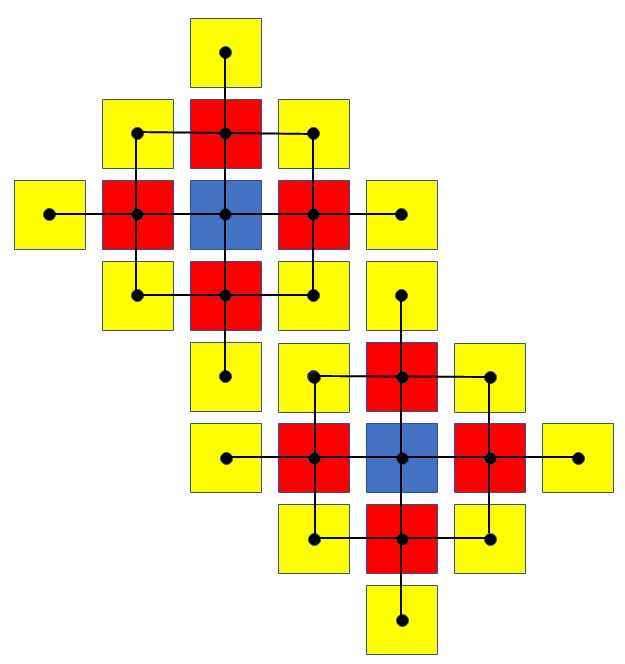
\includegraphics[width=0.99\linewidth]{Chapters/ProjROMs/Images/load_balancing_withEdgeCuts_noSyms.png}
    \end{minipage}
    \centering
    \begin{minipage}{0.45\linewidth}
        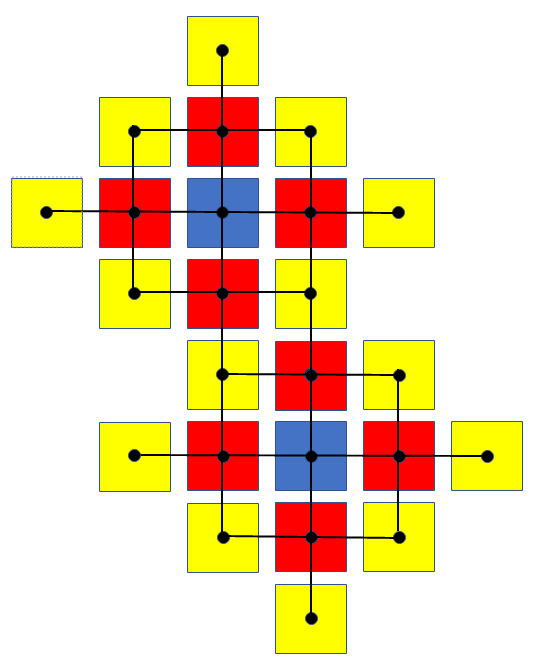
\includegraphics[width=0.99\linewidth]{Chapters/ProjROMs/Images/load_balancing_noEdgeCuts_noSyms.png}
    \end{minipage}
    \caption{\label{fig:edgeCuts}Mesh (graph) partitioning for load balancing. Some graph edges at finite volume cell faces can be excluded (left), while others are required (right).}
\end{figure}

As will be shown in Chapter~\ref{chap:CavityAndCVRC}, this approach to sample mesh partitioning can even lead to meshes which require zero MPI communications (besides collective operations). This occurs when sampling produces a number of small, disjoint graphs, i.e., individual graphs distributed in space which are not connected by any edges. On the other hand, fewer large, contiguous graphs arising from clustered sampling tend to result in fewer total nodes and smaller partition sizes, though they generally require more edge cuts to effectively load balance. The sparse sampling strategy can have a significant effect on this balance, as will be discussed in Chapter~\ref{chap:CavityAndCVRC}.

%%%%%%%%%%%%%%%%%%%%%%%%%%%%%%%%%

% We now frame these sampling strategies in the context of the discussion in Section~\ref{sec:sampCoupledEqs}, where we describe that sampling individual degrees of freedom requires that additional, auxiliary degrees of freedom also be sampled in order to correctly compute the approximated non-linear function. Much of the sampling theory does not discuss this nuance, instead treating all degrees of freedom impartially. Other works~\cite{carlberg_gnat}, on the other hand, modify their greedy sampling methods such that the algorithm selects the \textit{mesh element} whose associated degrees of freedom are, in the aggregate, optimal at each greedy iteration. This accounts for the fact that if any degree of freedom is selected at a mesh element, all degrees of freedom at that mesh element must be sampled. As those additional degrees of freedom can be considered a sunk cost, assessing their contribution to the greedy selection metric provides a more complete description.

% The present  work implements a slightly different approach. At each sampling iteration, only greedy selection metrics for individual degrees of freedom are considered. However, once a single degree of freedom is selected and the associated canonical unit vector is appended to $\sampMat$, all other degrees of freedom associated with this same mesh element are also appended to $\sampMat$. These additional degrees of freedom are then excluded from selection in subsequent sampling iterations. Thus, each iteration of a given sampling algorithm selects all degrees of freedom at a single mesh element, but does not consider the contribution of all of those degrees of freedom in the greedy selection metric. In implementing these algorithms, a sampling rate percentage $\alpha \in [0, \; 1]$ of the total mesh elements to sample is specified, and each sampling iteration selects the degrees of freedom associated with a single mesh element until the desired percentage of mesh elements is sampled. As a result, the total number of degrees of freedom sampled is $\numSamps = \alpha \times \numCells \times \numVars$. This approach is more similar to that taken by Zhou~\cite{Zhou1DTubularReac}. We take care to note that this approach is not optimal, and that the mesh element-based approach described by~\cite{carlberg_gnat} is logically a more principled approach to the greedy selection methodology. Future work will explore the performance differences between hyper-reduced ROMs using these two approaches.

% Prior work~\cite{carlberg_gnat, BloniganHypersonicROMs} has noted that it is important to sample at least  one mesh element at each inlet and outlet boundary to facilitate the communication of information from outside of the domain to the other sampled cells. Although this consideration is logical, it is not applied in this work. As will be seen later, this omission does not appear to affect the accuracy and robustness of the hyper-reduced ROMs presented. However, this may simply be the result of rather simple boundary conditions, namely fixed mass inflow and characteristic outflow conditions, with relatively minor influence on the domain interior during the examined time window. For more complex boundary conditions, such as those with artificial pressure forcing or varying mass flow rates, sampling boundary cells may prove to be more important.

